\chapter{Data generation}\label{ch:method}
In this chapter, we outline the process of generating the data required for the data-driven methods, which is a crucial part of the project.
We generate all the data ourselves using our numerical soler, and the quality and relevance of the data directly impact the training and performance of the models.
We begin by detailing the data generation process for the 1D SWE using the FVM with fluxes determined from an exact Riemann solver.
Next, we describe the approach for generating data for the 1D LSWE in spherical coordinates.
We also present the methodology for data generation in the context of the 2D SWE.
Finally, we provide a brief introduction of how we plan to generate data for training a spherical Fourier neural operator (SFNO) for applications on a planetary scale.

\section{Data generation using the Finite Volume Method}\label{sec:data_generation_fvm}
In this section we clarify the process of generating data using our numerical solver, that is, the FVM.
The FVM is used to solve the 1D SWE, 1D LSWE on a sphere and the 2D SWE.
We specify the necessary information, such as the initial conditions, the domain, and the parameters used in the data generation process.

\subsection*{1D SWE with exact Riemann solver}
In this section, we present how the so-called true solution is found in the code by solving the Riemann problem exactly.
The true solution is found by solving the Riemann problem exact using a high-resolution grid, and distinguishing between the wetbed or drybed case, and also identifying the shock and rarefaction waves.
First we caculate the wave speeds for the left and right states, respectively, as
\begin{align*}
    c_L = \sqrt{g h_L}, \quad c_R = \sqrt{g h_R},
\end{align*}
which are used to determine the critical water height $h_{\text{crit}}$ as
\begin{align*}
    h_{\text{crit}} = (u_R - u_L) - 2(c_L + c_R).
\end{align*}
If either $h_L \leq 0$ or $h_R \leq 0$, we are in a drybed case.
If $h_{\text{crit}} \geq 0$, it indicates that the water depth is critical, and we are also in a drybed case.
If none of the above conditions are met, we are in a wetbed case.
Summarized:
\begin{align*}
    \begin{cases}
        \text{Dry-bed case} & \text{if }  h_L \leq 0, \quad  h_R \leq 0 \text{ or } h_{\text{crit}} \geq 0, \\
        \text{Wet-bed case} & \text{otherwise}.
    \end{cases}
\end{align*}
In a dry bed case, we first identify the location of the dry region, whether it is on the left, right, or in the middle, and then calculate the wave speeds accordingly.
In a wet bed case, we compute the characteristics $h_*$ and $u_*$ for the star region.
We then identify the shock and rarefaction waves, and calculate the wave speeds for the left and right states, respectively.
The process is illustrated in \autoref{fig:flowchart_true_solution}.
\begin{figure}[H]
    \centering
    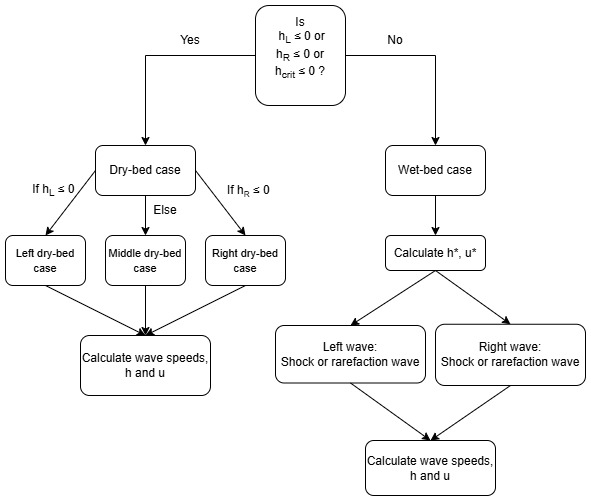
\includegraphics[width=0.8\textwidth]{C:/Users/Matteo/Shallow-Water-Equations/figs/flowchart_true_solution.jpg}
    \caption{Flowchart for generating the solution.}\label{fig:flowchart_true_solution}
\end{figure}
When generating the data, we need an initial condition for the water height $h$ and the velocity $u$.
In this study, we use the Gaussian function as the initial condition for the water height $h$.
That is, we define the initial condition for the water height as
\begin{align}\label{eq:1D_swe_ic_gaussian}
    h(x,0) &= a \exp{\left(\frac{-{(x-\mu)}^2}{2\sigma^2}\right)},
\end{align}
where $a$ is the amplitude of the Gaussian, $\mu$ is the center of the distribution, and $\sigma$ is the standard deviation.
We are working on the domain $x \in [0,1]$ m and the parameters are set to $a = 1$, $g = 9.81 m/s^2$ and $\sigma = 0.1$ m.
The value of $\mu$ is varied to generate different initial conditions, we generate data for $\mu = 0.3$ m and $\mu = 0.5$ m.
The initial conditions for the water height can be seen in \autoref{fig:data_generation_initial}.
\begin{figure}[H]
    \centering
    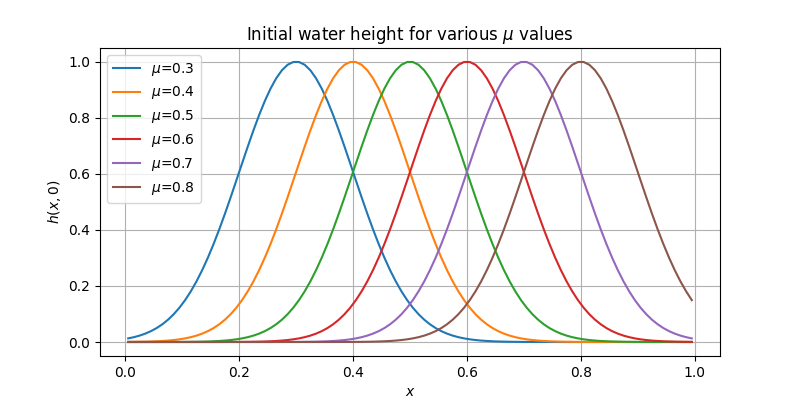
\includegraphics[width=0.5\textwidth]{C:/Users/Matteo/Shallow-Water-Equations/plots/data_generation_initial.png}
    \caption{The generated data has a Gaussian distribution for the initial water height, with $\mu = 0.3$ m and $\mu = 0.5$ m.}\label{fig:data_generation_initial}
\end{figure}
For the initial velocity $u$, we set it to zero, i.e., $u(x,0) = 0$ m/s, meaning that the water is initially at rest.
The solver is validated by comparing the results with known test cases, such as the dam break problem. 
We use a CFL number of $0.9$ and variable time steps.
The data is generate over the time interval $t = 0.0$ to $t_{\text{end}} = 1.0$ s.

\subsection*{Truncation error}
When generating data, it is essential to be aware of the truncation error.
Truncation erros arises from approximating the solution of the PDEs using a numerical method, in this case the FVM.
It specifically refers to the difference between the exact solution and the numerical approximation.
The critical question is: after a certain number of time steps, how significant is this error?
If the error becomes too large, it raises concerms about the reliability of the generated data.
Excessive truncation error could compromise the accuracy of the model trained on this data.
Therefore, we must carefully evaluate and mitigate these risks to ensure the data's quality.
To assess the truncation error, we generate a more accurate solution using a finer grid.
This high-resolution solution serves as a reference for evaluating the numerical approximation.
By comparing the high-resolution solution with the numerical solution, we gain insights into the error introduced by the approximation.

We generate a reference solution for solving the 1D SWE using $N = 1000$ grid points and compare it with the solution for $N = 100$ grid points at the final time step, $t = 1.0$ s.
The results are shown in \autoref{fig:1D_SWE_truncation_error}.
\begin{figure}[H]
    \centering
    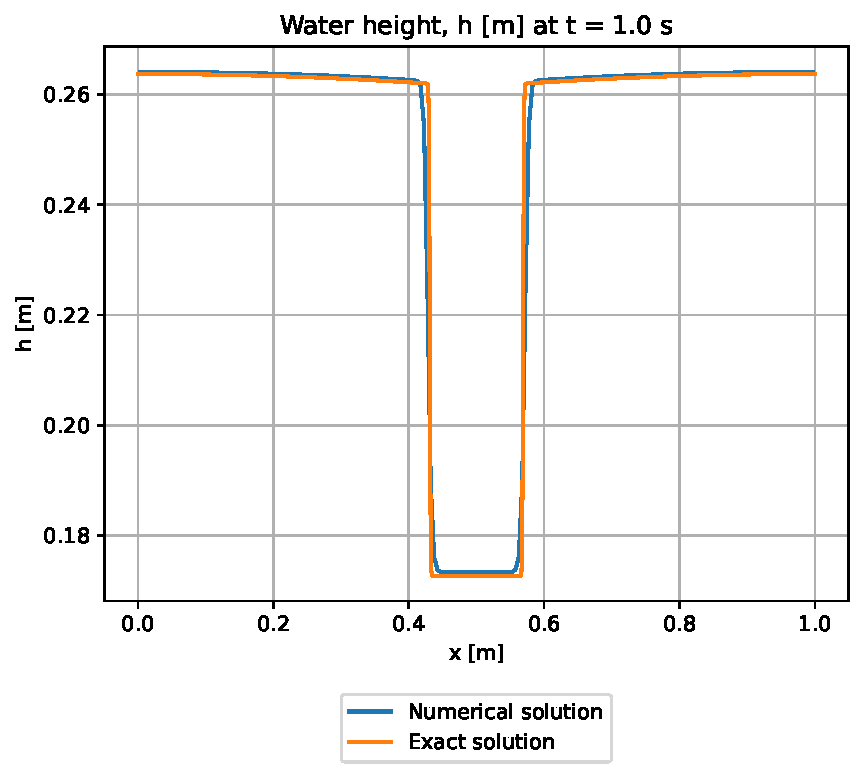
\includegraphics[width=0.5\textwidth]{C:/Users/Matteo/Shallow-Water-Equations/plots/truncation_error.pdf}
    \caption{Truncation error for the 1D SWE.}\label{fig:1D_SWE_truncation_error}
\end{figure}
The high-resolution solution (labelled as exact solution) and the low-resolution solution (labelled as numerical solution) are plotted in \autoref{fig:1D_SWE_truncation_error}.
We observe that there is a small difference between the high-resolution solution and the numerical solution, as the high-resolution solution has a more discontinuous behavior.
However, overall the two solutions are almost identical, indicating that the truncation error is negligible.
This suggests that the data generated using the FVM is of high quality and can be used for training the data-driven models.

\subsection*{1D LSWE on a sphere}
We also consider the 1D linearized shallow water equations in spherical coordinates, focusing on a circular domain.
The length of the domain corresponds to a full circle, $L = 2 \pi$ radians and is discretized into $N = 500$ points.
%The length of the domain corresponds to the circumreference of the circle, $L = 2\pi$ m, and is discretized into $N = 500$ points.
The initial condition for the water height $h$ is specified as a Gaussian function wrapped around the circle, expressed as:
\begin{align}\label{eq:1D_swe_spherical_ic}
    h(\theta, 0) &= a \exp \left( \frac{-{(\theta-\mu)}^2}{2 \sigma^2} \right),
\end{align}
where $h$ is the water height in meters, $a$ is the amplitude of the Gaussian, $\mu$ is the mean value, and $\sigma$ is the standard deviation.
The parameters are $a = 1$  and $\mu = \frac{\pi}{4}$ radians.
We generate data for varying values of $\sigma$ to investigate the effect of the standard deviation on the model performance.
The data is generated for $\sigma = \frac{\pi}{8}, \sigma = \frac{\pi}{16}$ and $\sigma = \frac{\pi}{32}$.
The initial velocity $u$ is set to zero, i.e., $u(\theta,0) = 0$ m/s.
The time step size is fixed and set to $\Delta t = 0.0025$ s.
The initial conditions for the three different $\sigma$ values can be seen in \autoref{fig:swe_spherical_1d_initial_conditions_sigmas}.
\begin{figure}[H]
    \centering
    \begin{subfigure}[b]{0.3\textwidth}
        \centering
        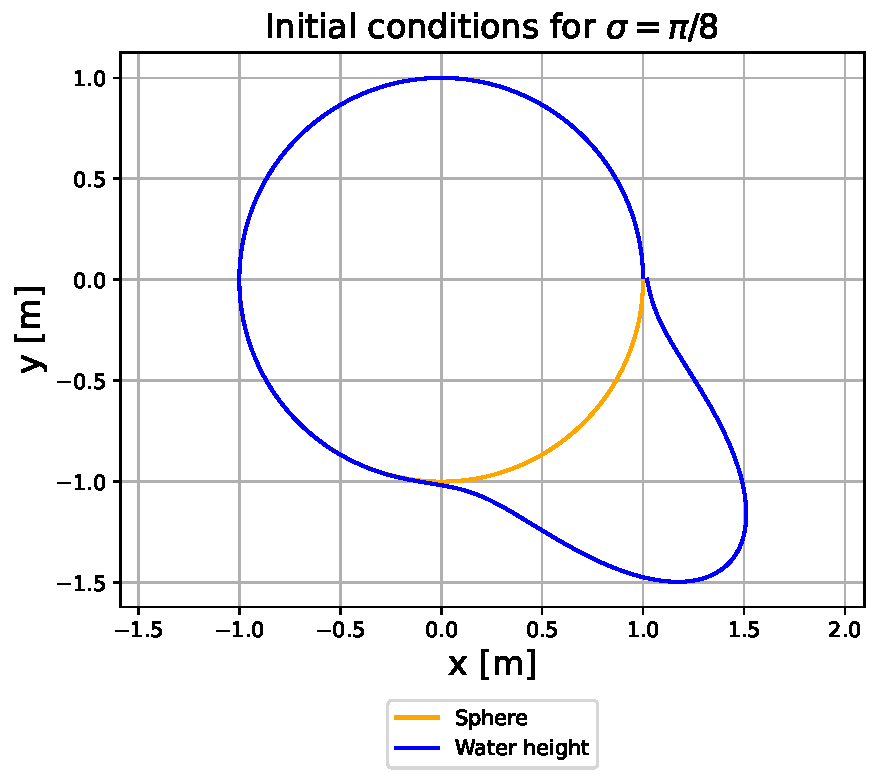
\includegraphics[width=\textwidth]{C:/Users/Matteo/Shallow-Water-Equations/plots/SWE-spherical-1d-initial_conditions_sigma1.pdf}
        \caption{$\sigma = \frac{\pi}{8}$.}\label{fig:swe_spherical_1d_sigma1}
    \end{subfigure}
    \hfill
    \begin{subfigure}[b]{0.3\textwidth}
        \centering
        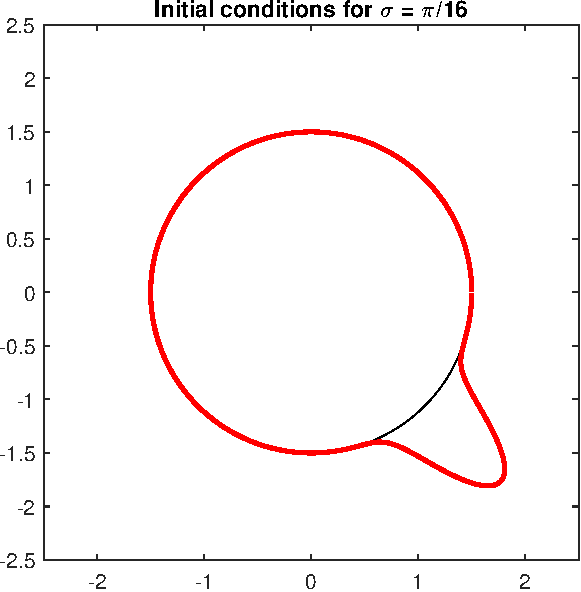
\includegraphics[width=\textwidth]{C:/Users/Matteo/Shallow-Water-Equations/plots/SWE-spherical-1d-initial_conditions_sigma2.pdf}
        \caption{$\sigma = \frac{\pi}{16}$.}\label{fig:swe_spherical_1d_sigma2}
    \end{subfigure}
    \hfill
    \begin{subfigure}[b]{0.3\textwidth}
        \centering
        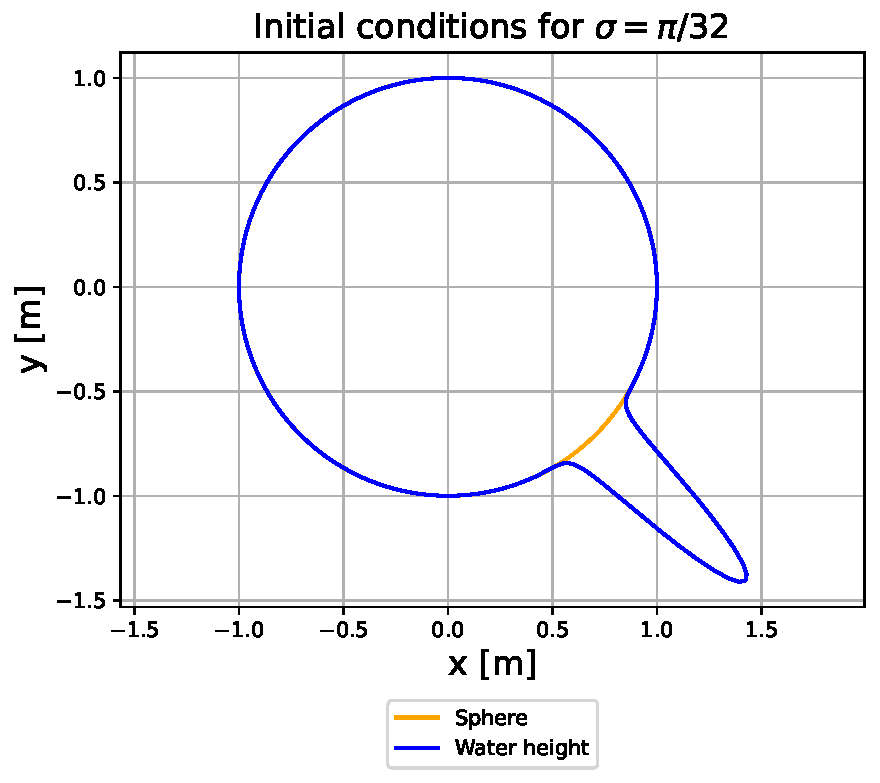
\includegraphics[width=\textwidth]{C:/Users/Matteo/Shallow-Water-Equations/plots/SWE-spherical-1d-initial_conditions_sigma3.pdf}
        \caption{$\sigma = \frac{\pi}{32}$.}\label{fig:swe_spherical_1d_sigma3}
    \end{subfigure}
    \caption{Initial conditions for the 1D LSWE in spherical coordinates for different \(\sigma\) values.}\label{fig:swe_spherical_1d_initial_conditions_sigmas}
\end{figure}
From \autoref{fig:swe_spherical_1d_initial_conditions_sigmas}, we observe that the standard deviation \(\sigma\) affects the width of the Gaussian function.
The smaller the $\sigma$, the narrower the Gaussian function, meaning the curves are steeper.
This is to test the different models abilities to handle steep gradients.
The data is generated from $t = 0.0$ to $t_{\text{end}} = 1.0$ s.

\subsection*{2D SWE}
%For the 2D SWE, we also use Gaussian functions with parametric extension~\cite{Gaussian} to generate the initial conditions.
For the 2D SWE, we also use the Gaussian function as initial condition for the water height $h$, but now in two dimensions:
\begin{align}\label{eq:2D_swe_ic_gaussian}
    h(x,y,0) &= h_0 + a \cdot \exp \left( -\frac{{(x-x_c)}^2 + {(y-y_c)}^2}{2\sigma^2} \right), 
\end{align}
where $h_0$ is the initial water height outside of the Gaussian, $a$ is the amplitude of the Gaussian in meters, $(x_c, y_c)$ is the center of the Gaussian in meters, and $\sigma$ is the standard deviation.
The domain is $x,y \in [0,40]$ m and is discretized into $N$ points in each direction.
We use the parameters $h_0 = 1$ m, $a = 2$ m, $(x_c, y_c) = (20 \text{m}, 20 \text{m})$, and $\sigma = 2$ m.
The initial velocity $u$ is set to zero, i.e., $u(x,y,0) = 0$.
The data is generated for different values of $N$ to investigate the effect of the grid resolution on the model performance.
To generate data like this also makes it possible to test the models abilities to transfer solutions to different grid resolutions.
The values of $N$ are $N = 64, N = 128$, and $N = 256$.
The time step size is variable and is set to satisfy the CFL condition, where the CFL number is set to $0.9$.
The initial conditions can be seen in \autoref{fig:2D_gauss_initial_condition}.
\begin{figure}[H]
    \centering
    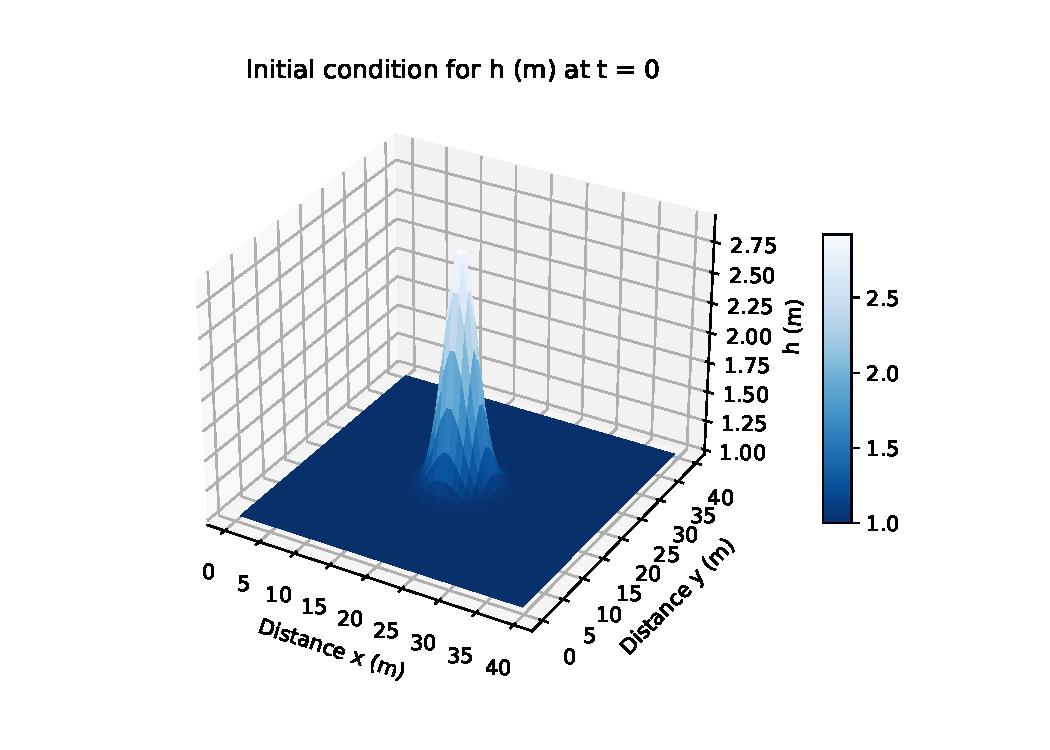
\includegraphics[width=0.8\textwidth]{C:/Users/Matteo/Shallow-Water-Equations/plots/2D_gauss_initial_condition.pdf}
    \caption{Initial condition for the 2D problem.}\label{fig:2D_gauss_initial_condition}
\end{figure}
To generate the data we use our FVM solver to solve the 2D SWE with the initial conditions given above, which is validated by comparing the results with known test cases.
The data is generated from $t = 0.0$ to $t_{\text{end}} = 10.0$ s.
In most of our test cases the models are using the data from $t = 0.0$ to $t_{\text{end}} = 5.0$ s, but we need the data to be generated for a longer time period to test the models ability to make long-term predictions.
Since we are making predictions beyond the data, the time step size is unknown, and we must work with a fixed time step size.
For generating data for long-term predictions, we employed a constant time step size of $\Delta t = 0.025$ s.
To ensure stability, the time step size must be sufficiently small.
To determine $\Delta t$, we analyzed the time step sizes used in the variable step data generation. 
By halving the smallest observed tme step size, we obtained $\Delta t = 0.025$ s.


